\documentclass[11pt,a4paper,oneside]{report}

\usepackage{amsmath}
\usepackage{graphicx}

\graphicspath{ {./images/} }


\begin{document}
\section{General two phase electric machine equations}

$\alpha\beta$ is a fixes coordinates frame, $dq$ is a rotating coordinates frame attached to a rotor.

\begin{center}
	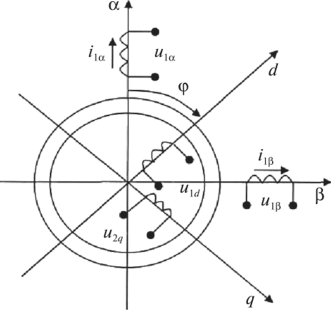
\includegraphics[scale=1]{electric_scheme}
\end{center}

Stator electric equations	
\begin{equation}
	\left\{
	\begin{split}
		& u_{s\alpha} = i_{\alpha}R_s+\frac{d\psi_{s\alpha}}{dt}\\
		& u_{s\beta} = i_{s\beta}R_s+\frac{d\psi_{s\beta}}{dt}
	\end{split}
	\right.
\end{equation}
where $u_{s\alpha}$ is a stator $\alpha$ phase voltage, $u_{s\beta}$ is a stator $\beta$ phase voltage, $i_{s\alpha}$ is a stator $\alpha$ phase current, $i_{s\beta}$ is a stator $\beta$ phase current, $\psi_{s\alpha}$ is a stator $\alpha$ phase flux linkage,  $\psi_{s\beta}$ is a stator $\beta$ phase flux linkage.

Rotor electric equations
\begin{equation}
	\left\{
	\begin{split}
		& u_{rd} = i_{rd}R_r+\frac{d\psi_{rd}}{dt}\\
		& u_{rq} = i_{rq}R_r+\frac{d\psi_{rq}}{dt}
	\end{split}
	\right.
\end{equation}
where $u_{rd}$ is a stator $d$ phase voltage, $u_{rq}$ is a stator $q$ phase voltage, $i_{rd}$ is a stator $d$ phase current, $i_{rq}$ is a stator $q$ phase current, $\psi_{rd}$ is a stator $d$ phase flux linkage,  $\psi_{rq}$ is a stator $q$ phase flux linkage.

Denote inductance as $L_{x,y}$, where $x$ means flux linkage that is created by the inductance, $y$ means current that creates flux linkage.

Flux equations

\begin{equation}
	\left\{
	\begin{split}
		& \psi_{s\alpha} = L_{s\alpha, s\alpha}i_{s\alpha}+ L_{s\alpha, s\beta}i_{s\beta}+L_{s\alpha, rd}i_{rd}+L_{s\alpha, rq}i_{rq} \\
		& \psi_{s\beta} = L_{s\beta, s\alpha}i_{s\alpha}+ L_{s\beta, s\beta}i_{s\beta}+L_{s\beta, rd}i_{rd}+L_{s\beta, rq}i_{rq} \\
		& \psi_{rd} = L_{rd, s\alpha}i_{s\alpha}+ L_{rd, s\beta}i_{s\beta}+L_{rd, rd}i_{rd}+L_{rd, rq}i_{rq} \\
		& \psi_{rq} = L_{rq, s\alpha}i_{s\alpha}+ L_{rq, s\beta}i_{s\beta}+L_{rq, rd}i_{rd}+L_{rq, rq}i_{rq} 
	\end{split}
	\right.
\end{equation}

or in matrix representation:

\begin{equation}
	\left[ 
	\begin{split}
		\psi_{s\alpha} \\ \psi_{s\beta} \\ \psi_{rd} \\ \psi_{rq}
	\end{split}
	\right]=L\left[
	\begin{split}
		i_{s\alpha} \\ i_{s\beta} \\ i_{rd} \\ i_{rq}
	\end{split}
	\right]
\end{equation}
where
\begin{equation}
	L=\left[
	\begin{array}{cccc}
		L_s & 0 & L_m\cos\theta & -L_m\sin\theta \\
		0 & L_s & L_m\sin\theta & L_m\cos\theta \\
		L_m\cos\theta & L_m\sin\theta & L_r & 0 \\
		-L_m\sin\theta & L_m\cos\theta & 0 & L_r
	\end{array}
	\right],
\end{equation}
$\theta$ is a rotor angle, $L_s$ is a stator inductance, $L_r$ is a rotor inductance, $L_m$ is rotor and stator cross inductance.

Momentum equation

\begin{equation}
	M=L_m\left[(i_{s\beta}i_{rd}-i_{s\alpha}i_{rq})\cos\theta-(i_{s\alpha}i_{rd}+i_{s\beta}i_{rq})\sin\theta\right]
\end{equation}

\section{Coordinates transformation}

Flux equations

\begin{equation}
	\left\{
	\begin{split}
		& \psi_{s\alpha} = L_si_{s\alpha}+L_mi_{rd}\cos\theta-L_mi_{rq}\sin\theta\\
		& \psi_{s\beta} = L_si_{s\beta}+L_mi_{rd}\sin\theta+L_mi_{rq}\cos\theta\\
		& \psi_{rd} = L_mi_{s\alpha}\cos\theta+L_mi_{s\beta}\sin\theta+L_ri_{rd}\\
		& \psi_{rq} = -L_mi_{s\alpha}\sin\theta+L_mi_{s\beta}\cos\theta+L_ri_{rq}
	\end{split}
	\right.
\end{equation}

In $\alpha\beta$ coordinates frame:
\begin{equation}
	\left\{
	\begin{split}
		& \psi_{s\alpha} = L_si_{s\alpha}+L_mi_{r\alpha}\\
		& \psi_{s\beta} = L_si_{s\beta}+L_mi_{r\beta}\\
		& \psi_{r\alpha} = L_mi_{s\alpha}+L_ri_{r\alpha}\\
		& \psi_{r\beta} = L_mi_{s\beta}+L_ri_{r\beta}
	\end{split}
	\right.
\end{equation}

In $dq$ coordinates frame:
\begin{equation}
	\left\{
	\begin{split}
		& \psi_{sd} = L_si_{sd}+L_mi_{rd}\\
		& \psi_{sq} = L_si_{sq}+L_mi_{rq}\\
		& \psi_{rd} = L_mi_{sd}+L_ri_{rd}\\
		& \psi_{rq} = L_mi_{sq}+L_ri_{rq}
	\end{split}
	\right.
\end{equation}

Momentum equation takes the form

\begin{equation}
	M = \psi_{s\alpha}i_{s\beta}-\psi_{s\beta}i_{s\alpha}.
\end{equation}

Rotor electric equations take the form

\begin{equation}
	\left\{
	\begin{split}
		u_{r\alpha} = i_{r\alpha}R_r+\frac{d\psi_{r\alpha}}{dt}+\omega\psi_{r\beta}\\
		u_{r\beta} = i_{r\beta}R_r+\frac{d\psi_{r\beta}}{dt}-\omega\psi_{r\alpha}
	\end{split}
	\right.
\end{equation}






	
\end{document}